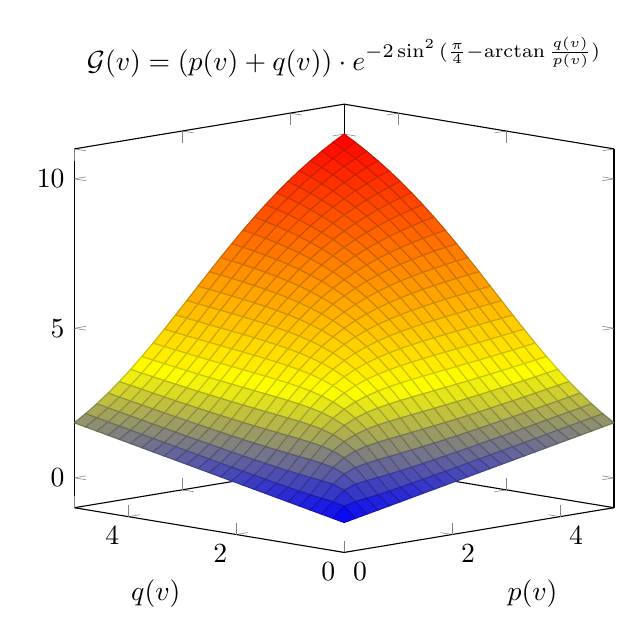
\begin{tikzpicture}[
    declare function={tf(\x)=(pi/4-rad(atan(\x)));},
    declare function={func(\x,\y)=sin(tf(\y/\x)*180/pi);}
]
\begin{axis}[
    view={315}{10},
    title={$
\mathcal{G}(v) = (p(v) + q(v)) \cdot e^{-2\sin^2{(\frac{\pi}{4} -
\arctan\frac{q(v)}{p(v)})}}$},
    xlabel=$p(v)$,
    ylabel=$q(v)$,
]

\addplot3 [
        surf,
        domain=0:5,
        domain y=0:5,
    ] {(x+y)*exp((-2)*(func(x,y))^2)};
\end{axis}
\end{tikzpicture}
